% questions.tex —— 1963 年·全国卷 · 题目内容片段（无答案）
% 由 tools/generate_projects.py 依来源总账自 1963/1963_数学真题_试题.md 生成，勿手改（改源 MD 后重跑）


\begin{gktip}
\textbf{题面说明}：固定 PDF 内页只标作“1963 年试题”，未载地区、科类、考试时长、总分、考试说明或逐题分值。本题库按原题顺序整理，现代 LaTeX 仅规范数学符号，不把缺失信息补成确定事实。
\end{gktip}

\gkpart{一、小题}

\begin{question}
\gkti{1}已知 $\tan\theta=\sqrt2$，求

\nopagebreak[4]
\[
\frac{\cos\theta+\sin\theta}{\cos\theta-\sin\theta}
\]

的值。

\end{question}
\begin{question}
\gkti{2}

（1） 求出复数 $1+\sqrt3i$ 的模数和辐角。

（2） 在直角坐标系 $XOY$ 所在的平面内，以 $A$ 点表示复数 $1+\sqrt3i$，把 $OA$ 绕着 $O$ 点按反时针方向旋转 $150^\circ$，设 $A$ 点到达的位置为 $B$，写出 $B$ 点所表示的复数的代数式。

\Needspace{0.4\textheight}
\end{question}
\begin{question}
\gkti{3}如图，$AB$ 为半圆的直径，$CD\perp AB$。已知 $AB=1$，$AC:CB=4:1$，求 $CD$。
\nopagebreak[4]
\begin{center}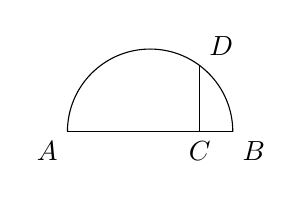
\begin{tikzpicture}[scale=2.1]
  \draw (0,0) -- (1,0);
  \draw (0,0) arc (180:0:0.5);
  \draw (0.8,0) -- (0.8,0.4);
  \node[below left] at (0,0) {$A$};
  \node[below right] at (1,0) {$B$};
  \node[below] at (0.8,0) {$C$};
  \node[above right] at (0.8,0.4) {$D$};
\end{tikzpicture}
\end{center}
\nopagebreak[4]
\end{question}
\begin{question}
\gkti{4}从二面角内任意一点向二面角的两个面作垂线，求证这两条垂线所决定的平面垂直于二面角的棱。（要求画图）

\end{question}
\begin{question}
\gkti{5}利用下列常用对数表，计算

\nopagebreak[4]
\[
23.28^{-1.1}
\]

常用对数表（原表右侧的数字为平均差栏；为适合 A4 黑白打印，整理为两张窄表，数据不变）：

\scriptsize

\begin{center}
\begingroup\setlength{\tabcolsep}{4pt}
\begin{tabular}{crrrrrrrrrr}
\toprule
$N$ & 0 & 1 & 2 & 3 & 4 & 5 & 6 & 7 & 8 & 9 \\
\midrule
23 & 3617 & 3636 & 3655 & 3674 & 3692 & 3711 & 3729 & 3747 & 3766 & 3784 \\
24 & 3802 & 3820 & 3838 & 3856 & 3874 & 3892 & 3909 & 3927 & 3945 & 3962 \\
25 & 3979 & 3997 & 4014 & 4031 & 4048 & 4065 & 4082 & 4099 & 4116 & 4133 \\
\bottomrule
\end{tabular}
\endgroup
\end{center}

\normalsize

常用对数表平均差栏：

\scriptsize

\begin{center}
\begingroup\setlength{\tabcolsep}{4pt}
\begin{tabular}{crrrrrrrrr}
\toprule
$N$ & 1 & 2 & 3 & 4 & 5 & 6 & 7 & 8 & 9 \\
\midrule
23 & 2 & 4 & 6 & 7 & 9 & 11 & 13 & 15 & 17 \\
24 & 2 & 4 & 5 & 7 & 9 & 11 & 12 & 14 & 16 \\
25 & 2 & 3 & 5 & 7 & 9 & 10 & 12 & 14 & 15 \\
\bottomrule
\end{tabular}
\endgroup
\end{center}

\normalsize

反对数表（同样将主体和平均差栏分开）：

\scriptsize

\begin{center}
\begingroup\setlength{\tabcolsep}{4pt}
\begin{tabular}{crrrrrrrrrr}
\toprule
$m$ & 0 & 1 & 2 & 3 & 4 & 5 & 6 & 7 & 8 & 9 \\
\midrule
.48 & 3020 & 3027 & 3034 & 3041 & 3048 & 3055 & 3062 & 3069 & 3076 & 3083 \\
.49 & 3090 & 3097 & 3105 & 3112 & 3119 & 3126 & 3133 & 3141 & 3148 & 3155 \\
.50 & 3162 & 3170 & 3177 & 3184 & 3192 & 3199 & 3206 & 3214 & 3221 & 3228 \\
\bottomrule
\end{tabular}
\endgroup
\end{center}

\normalsize

反对数表平均差栏：

\scriptsize

\begin{center}
\begingroup\setlength{\tabcolsep}{4pt}
\begin{tabular}{crrrrrrrrr}
\toprule
$m$ & 1 & 2 & 3 & 4 & 5 & 6 & 7 & 8 & 9 \\
\midrule
.48 & 1 & 1 & 2 & 3 & 4 & 4 & 5 & 6 & 6 \\
.49 & 1 & 1 & 2 & 3 & 4 & 4 & 5 & 6 & 6 \\
.50 & 1 & 1 & 2 & 3 & 4 & 4 & 5 & 6 & 7 \\
\bottomrule
\end{tabular}
\endgroup
\end{center}

\normalsize

\end{question}
\gkpart{二、大题}

\begin{question}
\gkti{6}解方程：

\nopagebreak[4]
\[
\sin3x-\sin x+\cos2x=0
\]

\end{question}
\begin{question}
\gkti{7}用 $1,2,3,4,7,9$ 组成没有重复数字的五位数，问：

（1） 这样的五位数一共有多少个？

（2） 在这些五位数中，有多少个是偶数？

（3） 在这些五位数中，有多少个是 $3$ 的倍数？

\end{question}
\begin{question}
\gkti{8}解方程组：

\nopagebreak[4]
\[
\begin{cases}
x^2-2xy-y^2=1,\\[2pt]
\sqrt{xy+3}=x.
\end{cases}
\]

（限定在实数范围内。）

\Needspace{0.4\textheight}
\end{question}
\begin{question}
\gkti{9}如图，线段 $CD$ 与 $\odot O$ 相交于 $A\text{、}B$ 两点，且 $AC=BD$，又 $CE\text{、}DF$ 分别与 $\odot O$ 相切于 $E\text{、}F$。求证：

\nopagebreak[4]
\[
\triangle OEC\cong\triangle OFD
\]
\nopagebreak[4]
\begin{center}\begin{tikzpicture}[scale=1.45,>=Stealth]
  \coordinate (O) at (0,0);
  \coordinate (C) at (-1.7,0);
  \coordinate (A) at (-0.72,0);
  \coordinate (B) at (0.72,0);
  \coordinate (D) at (1.7,0);
  \coordinate (E) at (-0.588,0.809);
  \coordinate (F) at (0.588,-0.809);
  \draw (O) circle (1);
  \draw[thick] (C) -- (D);
  \draw[thick] (C) -- (E);
  \draw[thick] (D) -- (F);
  \draw[dashed] (O) -- (E) (O) -- (F);
  \fill (O) circle (1.2pt) node[below] {$O$};
  \fill (A) circle (1.2pt) node[above] {$A$};
  \fill (B) circle (1.2pt) node[above] {$B$};
  \fill (C) circle (1.2pt) node[below left] {$C$};
  \fill (D) circle (1.2pt) node[below right] {$D$};
  \fill (E) circle (1.2pt) node[above left] {$E$};
  \fill (F) circle (1.2pt) node[below right] {$F$};
\end{tikzpicture}
\end{center}
\nopagebreak[4]
\Needspace{0.4\textheight}
\end{question}
\begin{question}
\gkti{10}如图，半径为 $1$ 的球内切于圆锥（即直圆锥），已知圆锥的母线与底面的夹角是 $2\theta$。

\Needspace{5\baselineskip}
（1） 求证圆锥的母线与底面半径的和是

\nopagebreak[4]
\[
\frac{2}{\tan\theta\left(1-\tan^2\theta\right)}
\]

\Needspace{5\baselineskip}
（2） 求证圆锥的全面积是

\nopagebreak[4]
\[
\frac{2\pi}{\tan^2\theta\left(1-\tan^2\theta\right)}
\]

（3） 当 $\theta$ 是什么值的时候，圆锥的全面积最小？（$\theta$ 用反三角函数表示。）

图中 $V$ 是圆锥的顶点，$VB$ 是母线，$O$ 是球心，$A$ 是球和圆锥底面的切点。
\nopagebreak[4]
\begin{center}\begin{tikzpicture}[scale=0.82,>=Stealth]
  \coordinate (V) at (0,4.5);
  \coordinate (B) at (-1.35,0);
  \coordinate (A) at (0,0);
  \coordinate (O) at (0,1);
  \coordinate (C) at (-0.49,1.64);
  \draw[thick] (V) -- (B) -- (A) -- cycle;
  \draw[dashed] (V) -- (A);
  \draw (O) circle (1);
  \draw[dashed] (-1.35,0) arc (180:360:1.35 and 0.28);
  \draw (B) arc (180:360:1.35 and 0.28);
  \draw[thick] (O) -- (A);
  \draw[thick] (O) -- (C);
  \draw pic[draw,angle radius=0.35cm,"$2\theta$" {shift={(0.08,0.12)}}]
    {angle=A--B--V};
  \fill (V) circle (1.3pt) node[above] {$V$};
  \fill (B) circle (1.3pt) node[below left] {$B$};
  \fill (A) circle (1.3pt) node[below right] {$A$};
  \fill (O) circle (1.3pt) node[right] {$O$};
  \fill (C) circle (1.3pt) node[left] {$C$};
\end{tikzpicture}
\end{center}
\nopagebreak[4]

\end{question}